\begin{figure*}[!htb]
    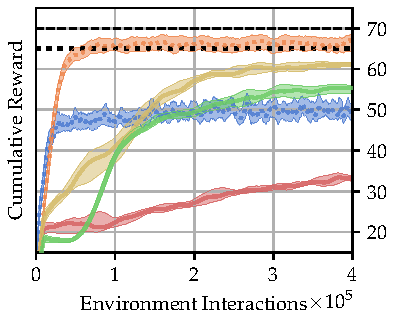
\includegraphics[width=0.315\textwidth]{figures/carla/scenario_1_time_steps_reward_results.pdf}
    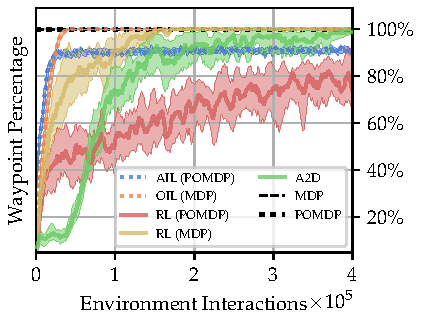
\includegraphics[width=0.335\textwidth]{figures/carla/scenario_1_time_steps_wpp_results.pdf}
    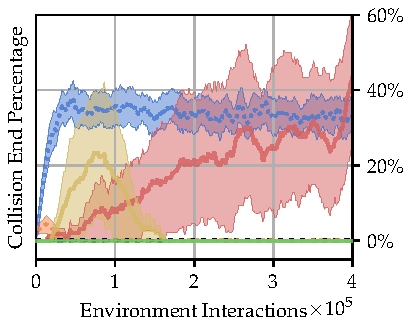
\includegraphics[width=0.33\textwidth]{figures/carla/scenario_1_time_steps_collision_results.pdf}
    \caption{Performance metrics for the AV scenario, introduced in Section \ref{sec:results}.  We show median and quartiles across ten random seeds.  Left: average cumulative reward.  Center: average percentage of waypoints collected, measuring progress along route.  Right: percentage of trajectories ending in a child collision.  Optimal MDP and POMDP solutions are shown by dashed and dotted lines respectively.  In methods marked as MDP the agent uses an omniscient compact state, including the child's state.  AIL (\emph{AIL (MDP)}) and RL (\emph{RL (MDP)}) learn a performant (high reward and waypoint percentage, low collision percentage) policy quickly and reliably.  In methods marked as POMDP the agent uses the high-dimensional monocular camera view.  Therefore, \emph{AIL} leads to a high collision, and the perception task makes RL in the POMDP (\emph{RL (POMDP)}) slow and variable (low reward and waypoint percentage, high collision percentage).  \emph{A2D} solves the scenario (high reward and waypoint percentage, low collision percentage) in a budget commensurate with the best-case convergence of \emph{RL (MDP)}.}
    \label{supp:fig:grid:a2dplot:results}
\end{figure*}

